\section{Basic Idea}
\label{Basic Idea}
Formally, a CDS of a graph $G$ is a set D of nodes with the following two properties:

(i) Any node in D can reach any other node in D using only the nodes that belong to D. 

(ii) Every node in G either belongs to D or is adjacent to a node in D. That is why D is called a dominating set of G.

Once the CDS is constructed broadcasting task is performed as follows:- if the source is in CDS then only the nodes in CDS need to forward the packet and the packet reaches all the nodes in the network because the nodes that are not in CDS must be neighbors of some node(s) in CDS. If the source is not in  CDS it can forward the packet to its neighbors and at least one of its neighbors is guaranteed to be in CDS. Thus the packet reaches one of the CDS nodes and all other nodes in CDS forward the packet like before.

 The main goal of this work is to construct a CDS 
 %in such a way so that when the nodes in CDS forward the message, the contentions among the nodes in CDS are as minimum as possible. In other word, a CDS will be constructed 
 that will intelligently select the nodes to reduce contention.  Upon receiving a packet from one node if two or more neighboring nodes try to rebroadcast the packet at the same time, there will occur contention. For example, consider the sample network of 7 nodes illustrated in Figure \ref{aa}.
 
\begin{figure}[h] 
    \centering
  \subfloat[]{%
       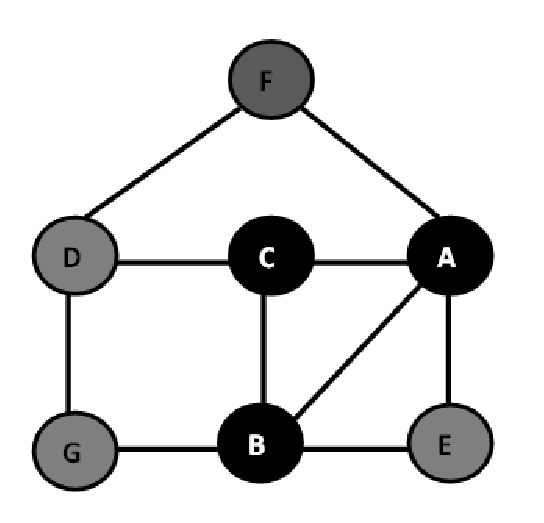
\includegraphics[width=0.5\linewidth]{Figures/mcds.eps}}
    \label{subfig1}\hfill
  \subfloat[]{%
        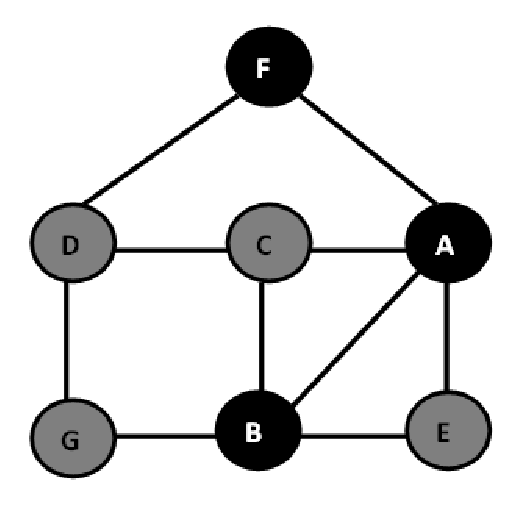
\includegraphics[width=0.5\linewidth]{Figures/cacds5.eps}}
    \label{subfig2}\\
  \caption{(a) CDS Construction with Contention, (b) CDS Construction without Contention}
  \label{aa} 
\end{figure}
Here one can easily see the following CDSs: 
 $$CDS = \{A,B,C\}, \{A,B,F\}, \{C,D,B\}, \{A,B,G\}, \{A,B,C,D\}$$
Among the above CDSs minimum size CDS  are as follows: 
$$MCDS = \{A,B,C\}, \{A,B,F\}, \{C,D,B\}, \{A,B,G\}$$
However the contention aware CDSs are only the followings:
$$CACDS = \{A,B,F\}, \{C,D,B\}, \{A,B,G\}$$
 
 In Fig \ref{aa}(a), if the CDS is constructed in traditional way, node A, B and C can be selected which will lead to contention problem. Because, upon receiving message from node A, if two of its neighbors node B and node C start to \emph{rebroadcast} it, they have to contend with each other first for gaining access to the shared channel as they are within the transmission range of each other. So, the selection of the nodes should be done intelligently to minimize this type of contentions. Figure \ref{aa}(b) presents a scenario, where node F is selected instead of node C to avoid the contention. The new heuristic designed for minimizing contention will never select {A,B,C} in order to avoid contention.
